\documentclass[a4paper,12pt]{report}

\usepackage{cmap}
\usepackage[T2A]{fontenc}
\usepackage[utf8]{inputenc}
\usepackage[russian]{babel}
\usepackage{amsmath,amsfonts,amssymb}
\usepackage{graphicx}
\usepackage{sidecap}
\usepackage{wrapfig}

\begin{document} 

\begin{titlepage} 

\begin{center} 

\large Федеральное государственное автономное образовательное учреждение высшего образования «Санкт-Петербургский государственный электротехнический университет «ЛЭТИ» им. В.И. Ульянова (Ленина)»
	
кафедра физики\\[5cm] 


\huge ОТЧЕТ\\ по лабораторной работе № 2\\[0.5cm] 
\large <<Исследование динамики свободных гармонических колебаний в поле силы тяжести>>\\[3.7cm]

\begin{minipage}{1\textwidth} 
    \begin{flushleft} 
        \emph{Автор:} Стукен В.А.\\
        \emph{Группа:} 2307\\
        \emph{Факультет:} ФКТИ\\
        \emph{Преподаватель:} Харитонский П.В. 
    \end{flushleft} 
\end{minipage} 

\vfill 

Санкт-Петербург, 2022\\
{\large \LaTeX} 

\end{center} 

\thispagestyle{empty} 
\end{titlepage} 

\section*{Работа №2 "Исследование динамики свободных гармонических колебаний в поле силы тяжести"}

\begin{wrapfigure}{r}{0.2\textwidth}
    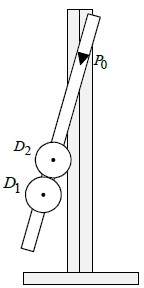
\includegraphics[width=0.2\textwidth]{ust.jpg}
    \label{ris:image}
\end{wrapfigure}

\par
\textit{Цель работы:} изучение закономерностей колебательного движения тела в однородном поле силы тяжести;
исследование процессов превращения энергии в консервативных системах; определение момента инерции физического маятника.

\textit{Приборы и принадлежности: } физический маятник;
секундомер; масштабная линейка, чертежный треугольник.

Конструкция оборотного маятника представлена на рис.1. На стержне 1 закреплены два диска - $D1$ и $D2$. Маятник может быть подвешен на кронштейне к легкой
призме, трение в которой пренебрежимо мало.

\section*{Исследуемые закономерности}

\par
Физический маятник - это тело с распределенной массой или система тел, ось вращения которого расположена выше центра масс маятника. Относительно этой оси маятник колеблется с периодом
\[T_0 = 2\pi\sqrt{\frac{I}{mgx_c}} = 2\pi\sqrt{\frac{l_0}{g}} \eqno{(1)}\]
где для составного маятника $m = \Sigma m_i$ - масса маятника, $x_c = \frac{1}{m}\Sigma m_{i}x_{ci}$ - положение его центра масс относительно оси вращенияl,
$I = \Sigma I_i$ полный момент инерции маятника, $I_i = I_{0i} + m_ix_{ci}^2$ - момент инерции i-го тела, расчитанный относительно оси вращения по теореме Штейнера,
$I_{oi}$ - момент инерции этого тела относительно его центра масс. Длина математического маятника, период которого совпадает с периодом колебаний физического маятника называется приведенной длиной физического маятника. 
Её можно найти как $l_0 = \frac{I}{mx_c} = \frac{gT_0^2}{4\pi^2}$. Ее можно определить экспериментально, если найти новую ось $O^{'}$, называемую осью качания, отнсительно которой маятник колеблется с тем же периодом $T_0$, что и отнсительно оси вращения $O$.
Расстояние между осями вращения и качания $OO^{'} = l_0$ и будет приведенной длиной физического маятника.

\par
Полный момент инерции маятника может быть представлен в виде:
\[I = I_0 + m\overline{x_c^2} \eqno{(2)}\]
где $I_0 = \Sigma I_{0i}, \overline{x_c^2} = \frac{1}{m}\Sigma m_ix_{ci}^2$ - средний квадрат положений центров масс системы тел, составляющих маятник.

\par
Если период колебаний маятника определен экспериментально, то из (1) можно найти момент инерции маятника:
\[I = mgx_{c}T_0^2/4\pi^2 .\eqno{(3)}\]

\par
\textit{Сохранение энергии гармонических колебаний.} Поскольку физический маятник, качающийся под действием силы тяжести, является консервативной системой, можно проанализировать процесс перехода потенциальной энергии маятника в кинетическую и обратно.

\par
Потенциальная энергия при достижении амплитудного значения угла отклонения равна:
\[W_{pm} = mgh_c = mgx_c(1-\cos{\varphi_m }) = 2mgx_c\sin^2{\frac{\varphi_m }{2}} \approx \frac{1}{2}mgx_c\varphi_m^2 \eqno{(4)}\]
где $h_c$ - высота поднятия центра масс маятника при его максимальном отклонении от положения равновесия, $x_c$ - положение центра масс маятника относительно его точки подвеса, $\varphi_m - $ максимальный угол отклонения маятника от положения равновесия.

\par
При малых углах отклонения маятника (до $20^{\circ}$) максимальная потенциальная энергия равна:
\[W_{pm}\approx \frac{1}{2}mgx_c\varphi_m^2\]

\par
Максимальная кинетическая энергия физического маятника:
\[W_{km} = \frac{I\omega_m^2}{2} = \frac{mgx_cT_0^2\omega_m^2}{8\pi^2} \eqno{(5)}\]
где момент инерции маятника выражен по формуле (3) через период его колебаний. Из закона сохранения полной механической энергии:
\[W = W_k + W_p = W_{km} = W_{pm} = const\]
можно найти максимальную уголовую скорость маятника при прохождении им положения равновесия $\omega_m = 2\pi\varphi_m/T_0.$

\newpage

\section*{Протокол измерений}

\begin{flushleft}
    
\resizebox{8cm}{!}{
    \begin{tabular}{|l|l|l|l|l|l|l|}
        \hline
            & 1 & 2 & 3 & 4 & 5 & $\theta$ \\
        \hline
        $t$,с  &   &   &   &   &   & \\ 
        \hline
    \end{tabular}
}

\resizebox{16cm}{!}{ 
    \begin{tabular}{|l|l|l|l|l|l|l|l|l|l|}
        \hline
           $l$ & $d$ &$D1 = D2$ & $h1=h2$ & $m$ & $\rho$ & $x_c$ & $x_1$ & $x_2$ & $x_3$\\
        \hline
               &     &          &         &     &        &       &       &       &\\ 
        \hline
    \end{tabular}
}
\end{flushleft}

\newpage
\section*{Ответы на вопросы}

\begin{itemize}
    \item \textbf{Вопрос №9:}
    	\textit{"Напишите уравнение для кинетической и потенциальной энергии физического маятника. Найдите полную энергию. Какой характер сил, действующих на качающееся тело, консервативный или диссипативный?"}
        \begin{itemize}
            \item Потенциальная энергия физического маятника равна:
            \[ E_p = mgh_c = mgx_c(1-\cos\varphi) \approx \frac{1}{2}mgx_c\varphi^2 \]
            \item Кинетическая энергия физического маятника равна:
            \[ E_k = \frac{I\omega^2}{2} \]
            \item Полная механическая энергия физического маятника равна:
            \[ E = E_p + E_k = \frac{1}{2}mgx_c\varphi^2 + \frac{1}{2}I\omega^2 \]
            \item Характер сил, действующих на тело консервативный, так как на него действует только сила тяжести, являющаяся консервативной силойю.
        \end{itemize}
    \item \textbf{Вопрос №23:}
        \textit{"Найдите отношение длин двух математических маятников, если отношение  периодов их колебаний равно 1,5."}
        \\По формуле периода математического маятника:
        \[ T = 2\pi\sqrt{\frac{l}{g}} \]
        Тогда:
        \[ \frac{T_1}{T_2} = \frac{2\pi\sqrt{\frac{l_1}{g}}}{2\pi\sqrt{\frac{l_2}{g}}} = \sqrt{\frac{l_1}{l_2}} = 1,5 \]
        Отсюда: 
        \[\frac{l_1}{l_2} = 2,25\]
\end{itemize}

\newpage

\section*{Ход работы:}

\subsection*{\textbf{Рассчитаем $t = \bar{t} \pm \Delta \bar{t} $:}}

\begin{flushleft}
$P = 95\%;$
$N = 5$
\[ \bar{t} = \sum_{i = 1}^{N} = 
\frac{t_1+t_2+t_3+t_4+t_5}{5} = 
\frac{11,99+12,22+12,24+12,31+12,12}{5} = 12,176 \, s \]

\[R = t_{\max} - t_{\min} = 12,31 - 11,99 = 0,32 \, s\]

\[\Delta t = \beta_{P,N} \cdot R = 0,51 \cdot 0,32 = 0,1632 \, s\]

\[\Delta \bar{t} = \sqrt{\Delta t^2 + \theta^2} = 0,1635 \, s\]

\[t = 12,18 \pm 0,16 \, s\]

\end{flushleft}

\subsection*{Рассчитаем период колебаний маятника: }
$P = 95\%;$
$n = 10$    

\[\bar{T_0} = \frac{\bar{t}}{n} = \frac{12,176}{10} = 1,2176 \, s \]
\[ a_t = \frac{dT_0}{dt}\bigg\vert_t = 0,1 \]
\[ \Delta\bar{T_0} = \sqrt{(a_t \cdot \Delta \bar{t})^2} = 0,01635 \, s \]
\[ T = 1,218 \pm 0,016 \, s\]

\subsection*{Рассчитаем момент инерции маятника:}

\[I = \bar{I} \pm \Delta \bar{I} \]
По формуле (3):
\[\bar{I} = \frac{mgx_{c}\bar{T_0}^2}{4\pi^2} = \frac{1,8 \cdot 9,8 \cdot 0,35 \cdot 1,2176^2}{4 \cdot 3,14^2} = 0,232 \, kg \cdot m^2\]
\[ a_{T_0} = \frac{dI}{dT_0}\bigg \vert_{T_0} =\frac{2mgx_{c}\bar{T_0}}{4\pi^2} = 0,3812\]
\[ \Delta \bar{I} = \sqrt{(a_{T_0} \cdot \Delta\bar T_0)^2} =  6,23\cdot 10^{-3} \, kg\cdot m^2\]
\[ I = (232 \pm 6,23)\cdot 10^{-3} \, kg\cdot m^2 \]

\subsection*{Рассчитаем полную механическую энергию маятника}

\[ E = E_{pm} = \frac{mgx_c\varphi_m^2}{2} = 0,5 \cdot 1,8 \cdot 0,35 \cdot (0,087)^2 = 0,0238 \, J\]

\subsection*{Рассчитаем приведенную длину маятника:}

\[ l_0 = \frac{\bar{I}}{mx_c} = \frac{0,232}{1,8 \cdot 0,35} = 0,368 \, m \]
\[ l_0 = \frac{g\bar{T_0}^2}{4\pi^2} = 0,368 \, m \]

\subsection*{Рассчитаем массы дисков $m_1$ и $m_2$ и стержня $m_3$:}

\[ m = \rho V = \rho s h = \rho \frac{\pi D^2}{4} h = \frac{8,7\cdot 10^{3}\cdot \pi \cdot (65,5\cdot 10^{-3})^2 \cdot 25,7\cdot 10^{-3} }{4} = 0,753 \, kg\]
Т.к $m_1 = m_2, D_1 = D_2 => m_1 = m_2 = 0,753 \, kg$
\[ m_3 = \rho V = \rho s l = \rho \frac{\pi D^2}{4} l = \frac{8,7\cdot 10^{3}\cdot \pi \cdot (10\cdot 10^{-3})^2 \cdot 0,61}{4} = 0,42 \, kg \]
\[m_{all} = \sum m_i = 0,753\cdot 2 + 0,42 = 1,925 \, kg\]
Из таблицы $m_{all} = 1,8 \, kg$

\subsection*{Рассчитаем положение центра масс маятника $x_c$:}

\[ x_c = \frac{1}{m}\sum m_i x_i = \frac{0,753\cdot 0,365 + 0,753\cdot 0,435 + 0,42 \cdot 0,245 }{1,925} = 0,366 \, m \]

\subsection*{Рассчитаем по теореме Штейнера момент инерции всех тел а также полный момент инерции маятника:}

\[ I_0 = \frac{mgR^2}{2} = \frac{mgD^2}{8} = \frac{0,753 \cdot 9,8 \cdot (65,5 \cdot 10^{-3})^2}{8} = 3,957 \cdot 10^{-3} \, kg\cdot m^2 \]
\[ I = \frac{m_1gR^2}{2} + m_1x_1^2 + \frac{m_2D^2}{8} + m_2x_2^2 + \frac{1}{3}m_3l^2 = 3,957\cdot 10^{-3} + 0,1 + 3,957\cdot 10^{-3} + 0,14 + 8,4\cdot 10^{-3} = 0,26 \, kg\cdot m^2\]
Сравнивая данное значение со значением полученным экспериментально\\
($I = (232\pm6,23)\cdot 10^{-3}$) видим, что значения очень близки.

\subsection*{Вывод:}
В ходе лабораторной работы я изучил закономерности колебательного движения тела в однородном поле силы тяжести, исследовал процессы превращения энергии в консерватиных системах, вычислил полную механическую энергию системы тел, а также определил момент инерции физического маятника.

\end{document} 